\documentclass[conference]{IEEEtran}
\usepackage[T1]{fontenc}
\usepackage{graphicx}
\usepackage{booktabs}
\usepackage{amsmath}
\usepackage{url}
\usepackage{xcolor}
\usepackage[hidelinks]{hyperref}

% Generated by analysis/make_paper_assets.py -- do not edit.
\newcommand{\ExpRuns}{144}
\newcommand{\ExpRequests}{258,046}
\newcommand{\ExpCPU}{M2}
\newcommand{\ExpCores}{8}
\newcommand{\ExpRAMGiB}{16}
\newcommand{\ExpPython}{3.12.13}
\newcommand{\ExpLiboqs}{0.16.0}
\newcommand{\ExpCommit}{30e6fb9}
\newcommand{\OvhPutSmallPoneBtwo}{-14.2}
\newcommand{\OvhPutSmallPoneBone}{-0.2}
\newcommand{\OvhPutSmallRoneBone}{+0.2}
\newcommand{\LatPutSmallPone}{5.27}
\newcommand{\LatPutSmallRone}{5.29}
\newcommand{\OvhPutMidPoneBtwo}{-27.6}
\newcommand{\OvhPutMidPoneBone}{-21.2}
\newcommand{\OvhPutMidRoneBone}{-22.6}
\newcommand{\LatPutMidPone}{12.31}
\newcommand{\LatPutMidRone}{12.08}
\newcommand{\OvhGetSmallPoneBtwo}{-10.4}
\newcommand{\OvhGetSmallPoneBone}{+6.6}
\newcommand{\OvhGetSmallRoneBone}{+243.4}
\newcommand{\LatGetSmallPone}{2.62}
\newcommand{\LatGetSmallRone}{8.45}
\newcommand{\OvhGetMidPoneBtwo}{+1.0}
\newcommand{\OvhGetMidPoneBone}{+3.0}
\newcommand{\OvhGetMidRoneBone}{+90.9}
\newcommand{\LatGetMidPone}{8.04}
\newcommand{\LatGetMidRone}{14.90}
\newcommand{\ClientShareKESmall}{33}
\newcommand{\ClientShareSerSmall}{45}
\newcommand{\ClientShareAeadSmall}{5}
\newcommand{\KEShareSmall}{2.1}
\newcommand{\StorageShareSmall}{93.5}
\newcommand{\ClientShareKELarge}{3}
\newcommand{\ClientShareSerLarge}{3}
\newcommand{\ClientShareAeadLarge}{92}
\newcommand{\KEShareLarge}{0.1}
\newcommand{\StorageShareLarge}{97.0}
\newcommand{\MicroPoneEnc}{17.4}
\newcommand{\MicroPoneDec}{20.1}
\newcommand{\MicroRoneEnc}{91.9}
\newcommand{\MicroRoneDec}{6,126}
\newcommand{\MicroBtwoEnc}{250.1}
\newcommand{\MicroBtwoDec}{165.6}
\newcommand{\MicroPtwoEnc}{271.8}
\newcommand{\MicroRoneOverPone}{305}
\newcommand{\MicroHKDF}{4.8}
\newcommand{\MicroAESGiBs}{7.1}
\newcommand{\NOnePutReductionHundred}{8.5}
\newcommand{\NOnePutReductionTen}{4.2}
\newcommand{\NOneGetReductionHundred}{9.9}
\newcommand{\NOneGetReductionTen}{4.7}
\newcommand{\MemSmallest}{3}
\newcommand{\MemLargest}{51}
\newcommand{\MemLargestSize}{500}
\newcommand{\MemSmallestSize}{1}

\newcommand{\prelim}{\textsc{Preliminary}}
\definecolor{warnbg}{HTML}{FDF3E6}
\definecolor{warnfg}{HTML}{8A5200}

\begin{document}

\title{Benchmarking Post-Quantum Key Encapsulation in S3-Compatible Object Storage under Client Concurrency}

\author{\IEEEauthorblockN{Team 12 (author names to be added)}
\IEEEauthorblockA{Department and institution to be added}}

\maketitle

\noindent\colorbox{warnbg}{\parbox{\dimexpr\columnwidth-2\fboxsep}{\footnotesize\color{warnfg}
\textbf{\prelim{} sample draft.} Every measurement in this version comes from a single
development laptop (\ExpCPU, \ExpCores{} logical cores) with MinIO in a local container,
one repetition per configuration and seconds-long runs. Such data is excluded from reported
results by the project protocol. It is included only to exercise the analysis pipeline and
show the shape of the final paper. All figures, tables and quoted numbers are regenerated
from raw files by \texttt{analysis/make\_paper\_assets.py}; the final version will use
two dedicated Linux hosts and repeated, randomized runs.}}

\begin{abstract}
Large-scale quantum computers would break the RSA and elliptic-curve key establishment
that protects most encrypted cloud data today, and ciphertext stored now can be decrypted
later. NIST standardized ML-KEM (FIPS~203) as the replacement key-encapsulation mechanism,
but its cost has mostly been measured in isolation or inside TLS handshakes, not in the
per-object encryption path of cloud object stores under concurrent load. We build an
instrumented client-side envelope-encryption layer for an S3-compatible store (MinIO) in
which every object is protected by ML-KEM-768, HKDF-SHA256 and chunked AES-256-GCM, and we
compare it on an identical data path against no encryption, symmetric-only encryption,
RSA-4096 key transport, X25519, and a hybrid X25519+ML-KEM-768 mode. Every request is
decomposed into key-establishment, key-derivation, encryption, metadata and storage time.
We also evaluate bounded session amortization, in which one ML-KEM encapsulation protects
a capped number of objects with per-object derived keys. In \prelim{} development-laptop
runs, ML-KEM-768 key establishment cost \MicroPoneEnc\,\textmu s (encapsulation) and
\MicroPoneDec\,\textmu s (decapsulation) per object in Python, less than X25519 in the same
stack, while RSA-4096 decryption cost about \MicroRoneOverPone$\times$ more than ML-KEM
decapsulation and raised median GET latency for 1\,KiB objects by
\OvhGetSmallRoneBone\,\%; storage round trips accounted for \StorageShareSmall--\StorageShareLarge\,\%
of PUT time at every object size; and a session bound of 100 reduced
mean key-establishment time by \NOnePutReductionHundred$\times$ (PUT) under 8 concurrent
workers. Streaming kept client memory growth near \MemLargest\,MiB for objects up to
\MemLargestSize\,MiB.
\end{abstract}

\begin{IEEEkeywords}
post-quantum cryptography, ML-KEM, object storage, S3, envelope encryption, benchmarking
\end{IEEEkeywords}

\section{Introduction}
Cloud object stores keep data for years. An adversary who records encrypted objects or
key-exchange traffic today can decrypt them once a cryptographically relevant quantum
computer exists (``harvest now, decrypt later''). The standard response is to replace
RSA and elliptic-curve key establishment with post-quantum key-encapsulation mechanisms.
In August 2024 NIST published FIPS~203, standardizing ML-KEM (derived from
CRYSTALS-Kyber) and recommending ML-KEM-768 as the default parameter set~\cite{fips203}.

For object storage the question is practical. Every object stored with client-side
envelope encryption needs its own key establishment, a larger per-object ciphertext and
metadata record, and more client CPU. Whether this matters depends on object sizes,
the operation mix and how many clients compete for the same CPUs and storage servers.
Prior measurements concentrate on algorithm micro-benchmarks and on TLS handshakes;
cloud-storage proposals evaluate security properties and single-client encryption time
(\S\ref{sec:related}).

\textbf{Contributions.} This paper
(i) presents an instrumented, reproducible benchmark of per-object ML-KEM-768 envelope
encryption on an S3-compatible store, with six key-establishment modes on one data path,
stage-level latency decomposition, client and server resource sampling, and bounded
memory for objects of hundreds of MiB;
(ii) evaluates bounded session amortization of ML-KEM, including a variant whose bound
follows client utilization, as a performance versus compromise-scope trade-off; and
(iii) releases the artifact, whose validator refuses data with inconsistent timers,
checksums or session bounds. Bounded key reuse itself is established practice
(\S\ref{sec:related}); our claim is its application to ML-KEM roots and its quantified
trade-off, and the queue-aware variant as a candidate policy.

\section{Background}
\textbf{ML-KEM.} A KEM has three algorithms: key generation, encapsulation (which, given
the recipient's public key, outputs a ciphertext and a 32-byte shared secret) and
decapsulation. ML-KEM-768 targets NIST security category~3, with a 1{,}184-byte
encapsulation key, a 2{,}400-byte decapsulation key and a 1{,}088-byte
ciphertext~\cite{fips203}. Decapsulation uses \emph{implicit rejection}: a modified
ciphertext or a wrong key yields a pseudorandom secret instead of an error, so tampering
is detected later by the authenticated encryption.

\textbf{Envelope encryption.} A per-object data key encrypts the object; key establishment
protects that data key for the recipient. We derive keys with HKDF-SHA256~\cite{rfc5869}
and encrypt with AES-256-GCM, which requires nonce uniqueness per key~\cite{sp80038d}.

\textbf{Object stores.} S3-compatible stores expose PUT and GET of whole objects. We use
MinIO~\cite{minio}. Its community edition was archived in April 2026 and no longer
publishes images, so we compile the final community release from source; because all
cryptography is client-side, any S3-compatible store can be substituted.

\section{Related Work}\label{sec:related}
\textbf{Algorithm-level cost.} Library benchmarks such as those in liboqs~\cite{liboqs}
and comparative studies of ML-KEM versus RSA and ECC~\cite{rodriguez2025} quantify key
generation, encapsulation and decapsulation, and the larger key and ciphertext sizes.
They do not include storage, concurrency or end-to-end request latency.

\textbf{Transport security.} Hybrid key exchange in TLS~1.3~\cite{rfc8446}, with
combiners such as X-Wing~\cite{xwing}, protects data in transit; session resumption
amortizes the handshake across connections. Our work concerns keys protecting data at rest,
one per object, and holds transport security constant.

\textbf{Post-quantum cloud storage.} Prikutse et al.~\cite{prikutse2026} combine AES-256-GCM,
X25519+ML-KEM-768 and ML-DSA-65 for multi-file cloud storage and amortize signatures by
batch commitment. According to its abstract, that evaluation does not cover an S3 store,
concurrent clients or queueing behaviour.

\textbf{Bounded key reuse.} Amazon S3 Bucket Keys derive per-object data keys from a
time-limited bucket-level key and reduce key-service requests by up to
99\%~\cite{s3bucketkeys}; the AWS Encryption SDK caches data keys with age and message-count
limits~\cite{esdkcache}. Our session mode applies the same principle to ML-KEM-established
roots in client-side encryption. We found no prior load-adaptive bound; this search must be
repeated in the academic databases before submission.

\section{Threat Model and Design}
\textbf{Threat model.} The network and object store are honest-but-curious for
confidentiality and potentially malicious for integrity: an adversary may read, replace,
delete, reorder or replay stored ciphertexts and manifests. The adversary does not hold
the recipient's decapsulation key. Availability, traffic analysis and side channels in the
Python client are out of scope.

\textbf{Construction (mode P1).} For object identity
$I=(\mathit{tenant},\mathit{bucket},\mathit{key},\mathit{version})$ the client computes
$(C,S)\leftarrow\mathrm{Encaps}(ek)$ and
$K\leftarrow\mathrm{HKDF}(S,\mathit{salt},\text{``pqc-s3-object-v2''}\|0\|\mathit{ctx})$,
where $\mathit{ctx}$ is canonical JSON of $I$, the mode, algorithm names, chunk size,
chunk count, plaintext size, recipient key identifier and a hash of $C$. The object is
split into 4\,MiB chunks; chunk $j$ uses nonce $p\|\mathrm{be}_{64}(j)$ with a random
32-bit prefix $p$ and associated data $\mathit{ctx}\|j\|\ell_j\|\mathit{final}_j$.
Deletion, reordering, truncation, extension and cross-object splicing therefore fail
authentication. The ciphertext stream is uploaded first and a manifest holding
$\mathit{ctx}$, $C$, the salt and the prefix is written last as the commit record, so an
interrupted upload is never visible. Object versions are time-ordered UUIDv7 values.

\textbf{Comparison modes.} All encrypting modes share the HKDF and chunked AES-GCM path
(Table~\ref{tab:micro}): B0 stores plaintext through the same framing (raw storage and
harness cost); B1 derives keys from a pre-shared 32-byte key; R1 transports a random
32-byte secret with RSA-OAEP-4096~\cite{rfc8017}; B2 uses ephemeral-static
X25519~\cite{rfc7748}; P2 concatenates X25519 and ML-KEM-768 secrets. A reader must name
the mode it expects, so a planted plaintext object cannot downgrade P1.

\textbf{Bounded sessions (mode N1).} One encapsulation yields a root $S_r$; object $i$ uses
$K_i=\mathrm{HKDF}(S_r,\mathit{salt}_i,\text{``pqc-s3-session-v1''}\|0\|\mathit{ctx}_i)$,
with the session identifier, the object's sequence number and the bound authenticated in
$\mathit{ctx}_i$. A root protects at most $B$ objects and lives at most $T_{\max}$ seconds.
In the queue-aware variant,
$B_t=\mathrm{clip}(B_{\min},B_{\max},\mathrm{round}(B_{\min}+(B_{\max}-B_{\min})\hat\rho))$
with $\hat\rho$ an exponentially weighted estimate of the fraction of busy worker threads;
$B_t$ is fixed per session, so $B_{\max}$ and $T_{\max}$ are hard caps. A leaked root
exposes at most $B_{\max}$ objects; compromise of the recipient's decapsulation key exposes
all objects in both P1 and N1. Receivers cache decapsulated roots under their own caps and
reject objects whose authenticated sequence number exceeds them.

\section{Implementation}
The client is Python~\ExpPython{} using liboqs~\ExpLiboqs{} through liboqs-python
(\cite{liboqs,liboqspython}), built from a pinned release with only ML-KEM enabled, and
pyca/cryptography~\cite{pyca} for HKDF, AES-GCM, RSA and X25519. A test checks ML-KEM
interoperability with an independent implementation (OpenSSL via pyca) in both directions.
The storage path streams: memory stays bounded regardless of object size
(Fig.~\ref{fig:memory}). A multi-process runner realizes a concurrency level $N$ as exactly
$N$ worker threads over $\min(N,\text{cores})$ processes that start together after warm-up.
It records every request, including failures, with stage timers, and samples client
resources and MinIO's own process metrics once per second. A validator rejects a data set
if checksums fail, a record deviates from the schema, any request's stage times exceed its
total, a run's 99th-percentile unaccounted time exceeds 2\,\%, or an N1 session exceeds its
bound. The test suite has over two hundred tests, including tamper, replay, downgrade and
session-bound stress tests.

\section{Methodology}
\textbf{Testbed (\prelim).} One \ExpCPU{} laptop (\ExpCores{} logical cores,
\ExpRAMGiB\,GiB RAM) ran both the client and MinIO in a local container over loopback; code
at commit \texttt{\ExpCommit}. The final study uses two dedicated Linux hosts.

\textbf{Workload.} Object sizes 1\,KiB, 64\,KiB, 1\,MiB and 16\,MiB; 1, 4 and 16
concurrent workers; PUT and GET separately; modes B0, B1, R1, B2, P1 and P2; closed loop,
1\,s warm-up and 4\,s measured per run; mode order randomized within each block;
\ExpRuns{} runs and \ExpRequests{} measured requests. GET runs read pre-written objects.
The N1 experiment compares P1 with N1 at $B\in\{1,10,100\}$ for 1\,KiB objects at 1 and 8
workers. Key-establishment micro-benchmarks run in-process after warm-up with the garbage
collector disabled.

\textbf{Metrics.} \emph{Handshake overhead} is key-establishment plus key-derivation time
per object; \emph{throughput} is successful operations (or MiB) per measured second;
client CPU is the summed CPU of worker processes and CPU time per request; server CPU and
memory come from MinIO's metrics endpoint. With one repetition we report request-level
medians and tail percentiles; the final study uses independent repetitions as the unit of
analysis with bootstrap confidence intervals.

\section{Preliminary Results}\label{sec:results}
\textbf{Cryptographic cost in isolation.} Table~\ref{tab:micro} lists per-object key
establishment. ML-KEM-768 costs \MicroPoneEnc\,\textmu s to encapsulate and
\MicroPoneDec\,\textmu s to decapsulate. In the same Python stack, ephemeral-static X25519
cost \MicroBtwoEnc\,\textmu s (sender) and \MicroBtwoDec\,\textmu s (receiver): generating an
ephemeral key, the exchange and key serialization each cross the library boundary, and
per-call overhead dominates the curve arithmetic itself, which OpenSSL's own benchmark puts
near 30\,\textmu s on this machine. The ordering between ML-KEM and X25519 is therefore a
property of the implementations, not of the algorithms, and the final study will report
native (C-level) costs alongside. The hybrid P2 costs about the sum of its parts
(\MicroPtwoEnc\,\textmu s sender side). RSA-4096 encryption is cheap (\MicroRoneEnc\,\textmu s) but decryption
costs \MicroRoneDec\,\textmu s, about \MicroRoneOverPone$\times$ ML-KEM decapsulation, which
places RSA's cost on the GET path. HKDF costs \MicroHKDF\,\textmu s and AES-256-GCM runs at
about \MicroAESGiBs\,GiB/s on 4\,MiB chunks.

\begin{table}[t]
\caption{Per-object key establishment, Python level (\prelim, median of in-process runs)}
\label{tab:micro}
\centering\footnotesize
% Generated by analysis/make_paper_assets.py -- do not edit.
\begin{tabular}{lrr}
\toprule
Mode & Sender (µs) & Receiver (µs) \\
\midrule
B1 AES only & 0.1 & 0.1 \\
R1 RSA-4096 & 91.9 & 6126.4 \\
B2 X25519 & 250.1 & 165.6 \\
P1 ML-KEM-768 & 17.4 & 20.1 \\
P2 hybrid & 271.8 & 189.0 \\
N1, B=10 (amortized) & 1.0 & -- \\
N1, B=100 (amortized) & 1.0 & -- \\
\bottomrule
\end{tabular}

\end{table}

\textbf{End-to-end latency.} Fig.~\ref{fig:latency} shows median latency per mode with one
worker. The clearest effect is RSA-4096 on the read path: its median GET latency was
\OvhGetSmallRoneBone\,\% above B1 for 1\,KiB objects and \OvhGetMidRoneBone\,\% above
for 1\,MiB objects (Table~\ref{tab:latency}), consistent with its private-key operation.
For P1 the picture is dominated by noise: its median 1\,MiB PUT latency differed from B1
by \OvhPutMidPoneBone\,\% and from X25519 by \OvhPutMidPoneBtwo\,\%, and its GET latency by
\OvhGetMidPoneBone\,\% and \OvhGetMidPoneBtwo\,\%. Differences of this size, in either
direction, cannot come from cryptography, whose handshake is below half a millisecond
(Table~\ref{tab:latency}, column hs.); they are run-to-run variation from one short
repetition on a shared laptop. Separating a sub-millisecond effect from this variation is
exactly what the repeated, randomized final design is for.

\begin{figure*}[t]
\centering
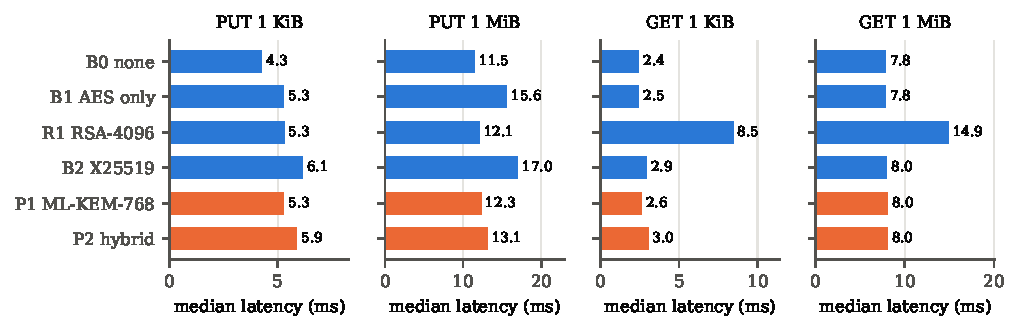
\includegraphics[width=\textwidth]{generated/fig-latency-by-mode.pdf}
\caption{Median end-to-end latency by mode, one worker (\prelim). Post-quantum modes in orange.}
\label{fig:latency}
\end{figure*}

\begin{table*}[t]
\caption{1\,MiB objects, one worker: median and p99 latency, handshake overhead (hs.) and change of the median relative to B1, all in ms except \% (\prelim)}
\label{tab:latency}
\centering\footnotesize
% Generated by analysis/make_paper_assets.py -- do not edit.
\begin{tabular}{lrrrrrrrr}
\toprule
Mode & PUT p50 & PUT p99 & PUT hs. & vs B1 \% & GET p50 & GET p99 & GET hs. & vs B1 \% \\
\midrule
B0 none & 11.48 & 16.56 & 0.001 & -26.5 & 7.81 & 12.07 & 0.000 & +0.1 \\
B1 AES only & 15.61 & 28.17 & 0.037 & -- & 7.80 & 17.19 & 0.029 & -- \\
R1 RSA-4096 & 12.08 & 19.26 & 0.162 & -22.6 & 14.90 & 20.78 & 6.833 & +90.9 \\
B2 X25519 & 17.01 & 28.53 & 0.375 & +9.0 & 7.96 & 11.65 & 0.252 & +2.0 \\
P1 ML-KEM-768 & 12.31 & 21.45 & 0.094 & -21.2 & 8.04 & 14.22 & 0.086 & +3.0 \\
P2 hybrid & 13.13 & 22.53 & 0.393 & -15.9 & 8.03 & 11.92 & 0.307 & +2.9 \\
\bottomrule
\end{tabular}

\end{table*}

\textbf{Where the time goes.} Fig.~\ref{fig:stages} decomposes P1 PUT time. Storage and
network account for \StorageShareSmall\,\% of mean PUT time at 1\,KiB and
\StorageShareLarge\,\% at 16\,MiB. Key establishment falls from \KEShareSmall\,\% to
\KEShareLarge\,\% over the same range: the direction the fixed-cost hypothesis predicts,
but small even for the smallest objects, because every PUT here costs two storage round
trips (data, then the committing manifest) against tens of microseconds of ML-KEM. Within
the client-side time, manifest handling (\ClientShareSerSmall\,\%) and key establishment
(\ClientShareKESmall\,\%) dominate for 1\,KiB objects, while AES-GCM takes
\ClientShareAeadLarge\,\% at 16\,MiB.

\begin{figure}[t]
\centering
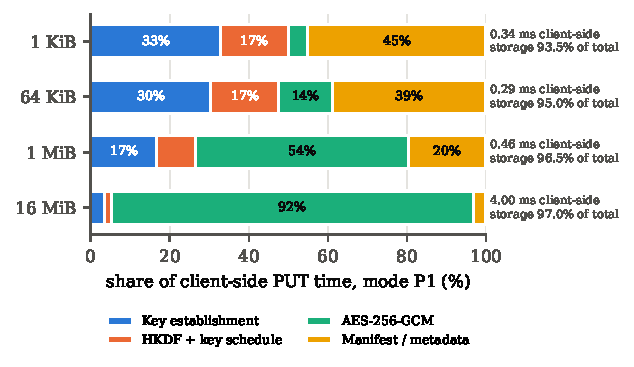
\includegraphics[width=\columnwidth]{generated/fig-stages-p1-put.pdf}
\caption{Composition of client-side P1 PUT time (all stages except storage), one worker; the storage share of total time is printed beside each bar (\prelim).}
\label{fig:stages}
\end{figure}

\textbf{Concurrency.} Fig.~\ref{fig:throughput} shows throughput from 1 to 16 workers for
B1, R1 and P1. Because client and server share one laptop, the curves reflect that
machine's saturation rather than the store's; Table~\ref{tab:resources} lists client and
server resources at 16 workers. Determining where the cryptographic client becomes the
bottleneck, and validating a queueing model against it~\cite{harchol2013}, requires the
two-host testbed.

\begin{figure*}[t]
\centering
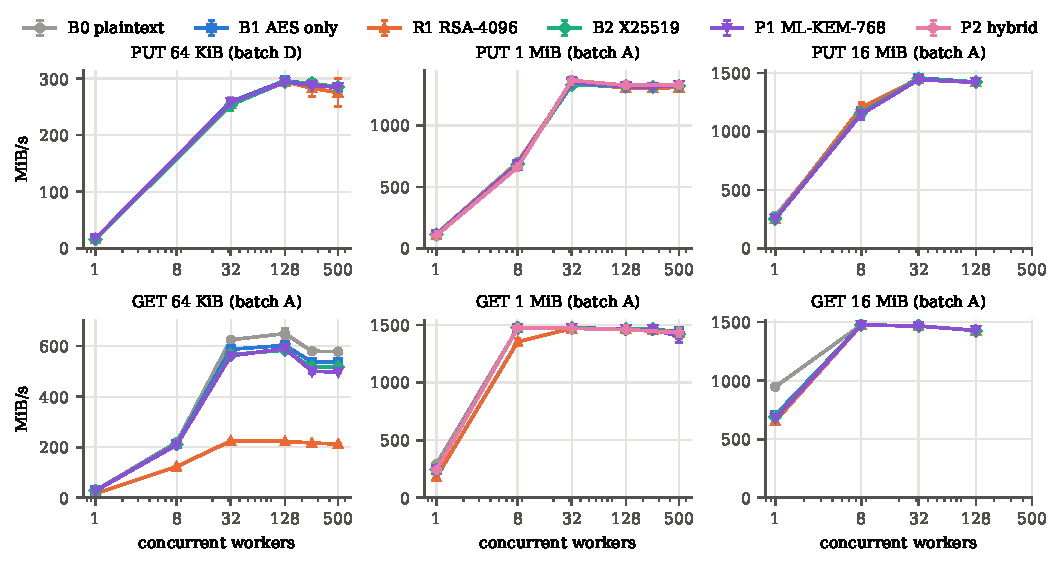
\includegraphics[width=\textwidth]{generated/fig-throughput.pdf}
\caption{Throughput versus concurrent workers for B1, R1 and P1 (\prelim; client and server on one host).}
\label{fig:throughput}
\end{figure*}

\begin{table}[t]
\caption{1\,MiB PUT with 16 workers: throughput and resources (\prelim)}
\label{tab:resources}
\centering\footnotesize
\resizebox{\columnwidth}{!}{% Generated by analysis/make_paper_assets.py -- do not edit.
\begin{tabular}{lrrrrr}
\toprule
Mode & MiB/s & CPU ms/req & Client CPU \% & Server CPU \% & Client RSS MiB \\
\midrule
B0 none & 102.4 & 3.34 & 35 & 185 & 544 \\
B1 AES only & 135.2 & 3.62 & 34 & 154 & 686 \\
R1 RSA-4096 & 129.6 & 3.85 & 43 & 183 & 587 \\
B2 X25519 & 134.4 & 3.93 & 48 & 195 & 697 \\
P1 ML-KEM-768 & 131.4 & 3.64 & 45 & 198 & 610 \\
P2 hybrid & 110.2 & 4.28 & 44 & 178 & 545 \\
\bottomrule
\end{tabular}
}
\end{table}

\textbf{Metadata.} The manifest per object (Table~\ref{tab:metadata}) grows with the
key-establishment ciphertext: 512 bytes for RSA-4096, 32 for X25519 and 1{,}088 for
ML-KEM-768 before base64 encoding. It exceeds the payload of a 1\,KiB object but is below
0.2\,\% of a 1\,MiB object.

\begin{table}[t]
\caption{Manifest size per object (\prelim, 1\,KiB PUT)}
\label{tab:metadata}
\centering\footnotesize
% Generated by analysis/make_paper_assets.py -- do not edit.
\begin{tabular}{lr}
\toprule
Mode & Manifest bytes \\
\midrule
B0 none & 529 \\
B1 AES only & 583 \\
R1 RSA-4096 & 1283 \\
B2 X25519 & 629 \\
P1 ML-KEM-768 & 2041 \\
P2 hybrid & 2092 \\
\bottomrule
\end{tabular}

\end{table}

\textbf{Bounded sessions.} Fig.~\ref{fig:n1} shows mean key-establishment time for N1 as the
session bound grows, with P1 as dotted reference lines. $B{=}1$ matches per-object ML-KEM,
as it must. With 8 workers, $B{=}10$ reduced mean key-establishment time by
\NOnePutReductionTen$\times$ for PUT and \NOneGetReductionTen$\times$ for GET relative to P1,
and $B{=}100$ by \NOnePutReductionHundred$\times$ and \NOneGetReductionHundred$\times$. The
compromise scope grows linearly with $B$; the final study plots this saving against scope
for $B$ up to 1000 and compares the queue-aware bound at equal offered load.

\begin{figure}[t]
\centering
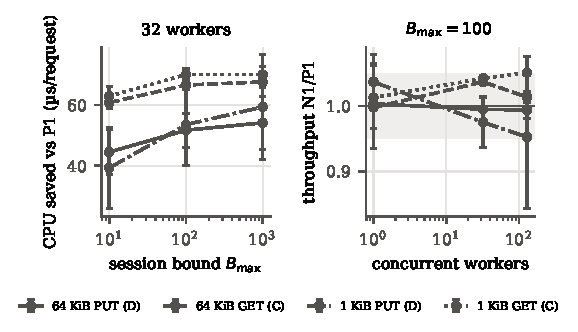
\includegraphics[width=\columnwidth]{generated/fig-n1.pdf}
\caption{N1 mean key establishment versus session bound $B$; dotted lines are P1 (\prelim).}
\label{fig:n1}
\end{figure}

\textbf{Memory.} Peak client memory growth for one PUT and GET was \MemSmallest\,MiB at
\MemSmallestSize\,MiB, rose while objects were smaller than the configured buffers
(4\,MiB chunks, 8\,MiB upload parts) and then stayed flat, reaching \MemLargest\,MiB at
\MemLargestSize\,MiB (Fig.~\ref{fig:memory}).

\begin{figure}[t]
\centering
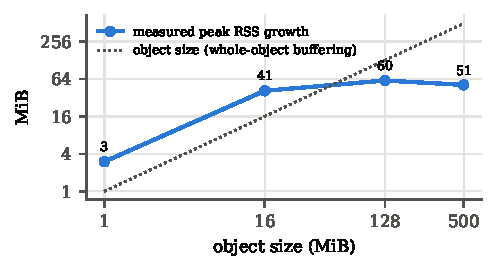
\includegraphics[width=\columnwidth]{generated/fig-memory.pdf}
\caption{Peak client memory growth for one PUT+GET versus object size (\prelim). The dotted line marks what whole-object buffering would need.}
\label{fig:memory}
\end{figure}

\section{Discussion}
Three observations are robust enough to shape the final study. First, ML-KEM-768 is not
expensive relative to the classical alternatives: its per-object cost is tens of
microseconds, below X25519 in our Python implementation (an implementation effect, see
\S\ref{sec:results}), while RSA-4096 places milliseconds of private-key work on every GET.
Second, against real storage round trips the per-object key-establishment cost is small at
every size; its share is largest for small objects, where the final study must resolve it
against run-to-run variation. Third, the size-dependent costs of post-quantum migration are metadata
bytes and client CPU per request, which become visible under concurrency, and session
amortization removes most key-establishment cost for small objects at a bounded
compromise scope.

\section{Threats to Validity}
This draft's numbers come from one laptop that also ran the store, from a single short
repetition per configuration and from a container over loopback; background load and
thermal effects are uncontrolled. The client is Python, so absolute costs include
interpreter overhead and differ from native or hardware-accelerated implementations.
MinIO ran as a single node without erasure coding, with a warm page cache for GETs.
liboqs is intended for prototyping, not production. The final study addresses the
measurement limitations with two dedicated Linux hosts, 5--10 independent repetitions,
longer runs, randomized order, bootstrap confidence intervals and pre-registered
hypotheses.

\section{Conclusion}
We built and validated an instrumented, reproducible benchmark of post-quantum envelope
encryption for S3-compatible object storage, covering six key-establishment modes on one
data path and a bounded session-amortization mode. Preliminary data indicates that
ML-KEM-768 adds tens of microseconds per object, far less than RSA-4096 on the read path,
and that its relative impact shrinks as objects grow. The final evaluation will measure
scaling to 500 concurrent clients and 500\,MiB objects on dedicated hosts and validate a
queueing model of client saturation.

\section*{Artifact}
Code, configurations, the analysis script that generates every figure and number in this
paper, and a validator for raw data are in the project repository, organized following
ACM artifact guidelines~\cite{acmbadges}.

\bibliographystyle{IEEEtran}
\bibliography{references}

\end{document}
